\section{Literatür Taraması, Özetler ve Pazar Araştırması}
Lorem ipsum dolor sit amet, consectetur adipiscing elit, sed do eiusmod tempor incididunt ut labore et dolore magna aliqua. Ut enim ad minim veniam, quis nostrud exercitation ullamco laboris nisi ut aliquip ex ea commodo consequat. Duis aute irure dolor in reprehenderit in voluptate velit esse cillum dolore eu fugiat nulla pariatur. Excepteur sint occaecat cupidatat non proident, sunt in culpa qui officia deserunt mollit anim id est laborum.



\subsection{E-Posta, SMS ve Push Notification: Hangisi Daha Etkili}
Makalede bahsedilen bildirim kanallarının efektiflikleri karşılaştırılıyor. Bu kanalların hızların, maliyetleri, kullanıcının bildirimi açma oranları gibi faktörler ele alnıyor. Makelde verilen istatiklerin bir kısmı aşşağıdaki tablodan incelenebilir.\cite{socilamediatoday}
\begin{center}
\begin{tabular}{ c | c | c | c }
 Yöntem & E-Posta & SMS & Push Bildirim \\ 
 Ulaşım Süresi & Yavaş & Anında & Anında  \\  
 Açma Oranı & 0.23(Endüstriye Bağlı) & 0.90 & 0.90  \\
 Maliyet & Orta & Yüksek & Düşük \\
 Ulaşılabilirlik & Orta & Yüksek & Orta \\
 Malware Olasığı & Yüksek & Düşük & Düşük \\
 Spam Oranı & Yüksek & Yükse & Düşük \\
 Abonelikten Çıkış Oranı & 0.20-0.50(Endüstriye Bağlı) & 0.60 & 0.40 
\end{tabular}
\end{center}

\subsection{İşletmeler İçin Toplu SMS'in Önemi}
Toplu SMS yöntemleri ile dünyanın her yerine ulaşma imkanı olduğununa değiniliyor. İnsanların \%90'nın gelen SMS'leri ilk 3 saniye içerisinde okuma ihitmalinin aşırı derecede yüksek olduğu söyleniyor. Toplu SMS sistemlerindeki "Aplication-to-Person" (A2P) kullanım kolaylığına dikkat çekiliyor. Özellikle bulut sistemlerindeki entegrasyon kolaylığına değiniliyor.\cite{clickatell} Avantajları 3 madde de özetleyecek olursak:
\begin{itemize}
  \item Global olarak erişim kolaylığı
  \item SMS Fiyatlandırmısanın Avantajları
  \item Kolay sistem entegrasyonu
\end{itemize}
\subsection{API Nedir}
Basit terimler ile Application Programming Interface (API) uygulamaların birbirleriyle etkileşmesini sağlaya yarar. API'ler web tabablı verilere(JSON veya XML) ulaşımda, bu verilerin değiştirilmesinde ve yeni verilen eklenmesinde kullanılır. Misal olarak Twitter'ın API'si sayesinde başka uygulamalardan Twitterin verisine erişim sağlanabilir.\cite{whatisapi}
\subsection{JavaScript Ne İçin Kullanılır}
Java script genelde web tabanlı uygulamar ve web tarayıcılarının programlanmasında kullanılır. Bunların yanısıra sunucularda ve gömülü sistemlerin kontrolünde de kullanılır. Ama en popüler kullanım sebebi web sitesi araclığıyla interaktif bir arayüz sağlanabilmesidir. Ayrıca JavaScript web tarayıcılarının "native" olarak anladığı tek programlama dilidir.\cite{whyjs}
\subsection{Javascript Framework: React}
React açık kaynak bir JavaScript kütüphanesidir ve Single-Page uygulamalar için kullanıcı arayüzü geliştirmede kullanılır. Facebook tarafından ilk defa kullanılmıştır. JSX adı verilen özel bir syntax'ı vardır. Bu syntax sayesinde hem JavaScript vs HTML'i karaşık olarak kullanma imkanı sunar. Hem iOS hem Android hemde Web uygulamarında kodun tekrar kullanımına olanak sağlar.\cite{react}
\subsection{TCP (Transmission Control Protocol) }
TCP bir network üzerindeki cihazlar için bir veri alışverişi standartıdır. 1973'de bilgisayar bilimcisi Robert E. Kahn ve Vinton G. Cerf tarafından bir araştırma makalesinde ilk defa bahsedilmiştir. Son versiyonu 2014 yılında RFC 7324'de\cite{RFC} tanımlanmıştır. TCP'nin şuan kullanımda olan haliyle iki taraflı veri alışverişine olanak sağlar. Tüm veri kayıpları otomatik olarak tespit edilir ve düzeltilir. Bu sebepten dolayı TCP güvenilir protokol olarak adlandırılır. TCP/IP protokol kavramlarıda bütünleşik olarak IP(Internet Protocol)'ünü kasıt ederek kullanılır. 
\newline
\newline
TCP yazılımı web browserler ve sunucular tarfında kontrol edilir. Her bağlantı kaynağı açıkca bitiş noktalarını(end points, server-client) açıkca tanımlamaldır. Hangi tarafın hangi rolü(server yada client) üstenldiği önemli değildir. TCP yazılımına he endpoint için bir çift IP adresi ve port sağlanması yeterlidir(socket ve 2-tuple).




\begin{figure}[h]
    \centering
    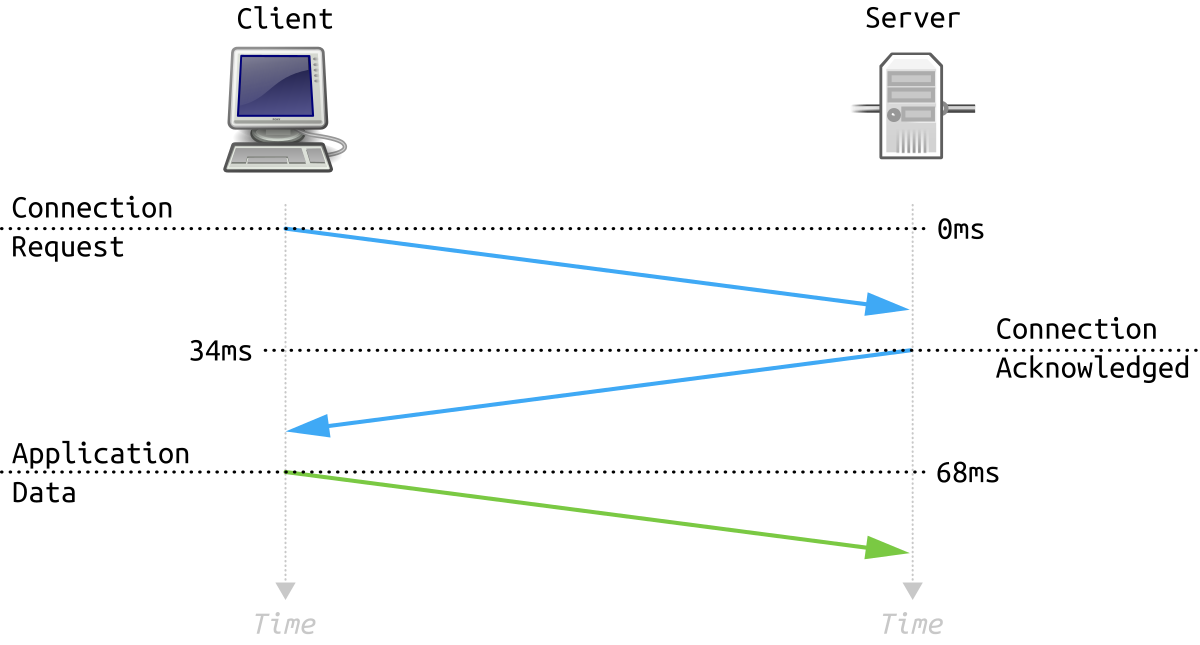
\includegraphics[width=\textwidth]{Report/images/tcp.png}
    \caption{TCP 3-Way Handshake yöntemiyle bağlantı sağlama süreci}
    \label{fig:mesh1}
\end{figure}


\subsection{Websocket Nedir}
Websocket tek bir TCP bağlantısı ile 2 yönlü iletişimi sağlar. Websocket geliştirmek için birçok dil ve kütüphane mevcuttur.\cite{websocket1}
\begin{itemize}
  \item ASP.Net Core: SignalR
  \item Node.js: Socket.IO, ws
  \item WebSockets, ws4py
\end{itemize}
Websocket'ler TCP'nin üzerine kurulan protokollerdir ve ayrıca gerçeklenmesi gerekir. Python'da bu mimariyi gerçekleyen kütüphaneler mevucttur. Yukardıki maddelerde verilen örneklere ek olarak Python'da Tornado kütüphanesi verilebilir\cite{websocket2}.

\subsection{Örnek Bildirim Motoru Mimarisi}
Bu makalade "OracleAS Wireless notification" sistemi mimarisi anlatılıyor. Bu mimari projede gerçeklenecek back-end kısmıyla bazı yönlerden parelellik göstediği için incelendi.
\noindent
Bu mimaride 3 tip bildirim tetikleme yöntemi mevcut.
\begin{itemize}
  \item Veri tetiklemesi
  \item Zaman tetiklemesi
  \item Lokasyon tetiklemsi
\end{itemize}
Veri tetikleme yöntemi bizim sistemimize en uygun olan yöntem. Bu yöntemde kullanıcının belirlediği kurallara göre yeni veri akışı olduğunda bildirim tetikleniyor. Örnek olarak bir hisse senedin belli bir fiyata ulaştığında bildirim gönderilmesi gibi.
\newline
\noindent
Zaman tetikleme yönteminde ise kullanıcı belirlene bir saatte ve yine isterse belirlediği kurallara göre bildirim alıyor. Örnek olarka kullanıcının her gün saat 15:00 borsa endeksini alması verilebilir.
\newline
\noindent
Lokasyon tetiklemesi kullanıcın veya kullanıcın takip ettiği kişinin o anki konumunu bir kural olarak kullanarak bildirim sağlanması. Örneğin kullanıcı belli bir dükkanın önündeyse veya işte veya evde değilse trafik durumuyla ilgili bildirim alması verilebilir.
\begin{figure}[!ht]
    \centering
    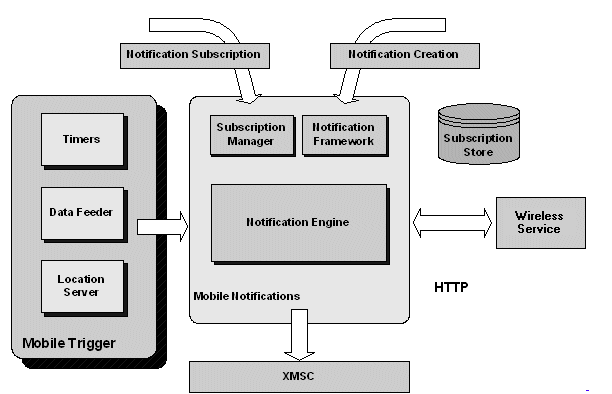
\includegraphics[width=\textwidth]{Report/images/notif.png}
    \caption{Örnek bildirim lojistik mimarisi\cite{notif}}
    \label{fig:mesh2}
\end{figure}


\subsection{Different ways to Authenticate a Web Application}
Lorem ipsum dolor sit amet, consectetur adipiscing elit, sed do eiusmod tempor incididunt ut labore et dolore magna aliqua. Ut enim ad minim veniam, quis nostrud exercitation ullamco laboris nisi ut aliquip ex ea commodo consequat. Duis aute irure dolor in reprehenderit in voluptate velit esse cillum dolore eu fugiat nulla pariatur. Excepteur sint occaecat cupidatat non proident, sunt in culpa qui officia deserunt mollit anim id est laborum.
\subsection{10. Özet}
Lorem ipsum dolor sit amet, consectetur adipiscing elit, sed do eiusmod tempor incididunt ut labore et dolore magna aliqua. Ut enim ad minim veniam, quis nostrud exercitation ullamco laboris nisi ut aliquip ex ea commodo consequat. Duis aute irure dolor in reprehenderit in voluptate velit esse cillum dolore eu fugiat nulla pariatur. Excepteur sint occaecat cupidatat non proident, sunt in culpa qui officia deserunt mollit anim id est laborum.
\subsection{Pazar Araştırması}
Lorem ipsum dolor sit amet, consectetur adipiscing elit, sed do eiusmod tempor incididunt ut labore et dolore magna aliqua. Ut enim ad minim veniam, quis nostrud exercitation ullamco laboris nisi ut aliquip ex ea commodo consequat. Duis aute irure dolor in reprehenderit in voluptate velit esse cillum dolore eu fugiat nulla pariatur. Excepteur sint occaecat cupidatat non proident, sunt in culpa qui officia deserunt mollit anim id est laborum.




